% 原书 p.133–p.140（PDF p.141–p.148）
% 第 5 章 5.5 节：指标（Indices）
% 注意：本文件不写 \chapter（章标题由 ch05a 负责）。p.141 上半页仍属 5.4 节（见 ch05b-s02.tex），
%       5.5 节自 p.141 中部开始。

\section{指标（Indices）}
% >>> p141

\begin{keytakeaways}
\begin{itemize}
  \item 几何图像：闭哈密顿轨道上的指标，本质上是度量该轨道上某个向量丛之非平凡性的整数；
        Floer 边界算子按指标差 $1$ 计数，因此指标是 Floer 理论中「维数计数」的替代品。
  \item 数学工具：转移映射与向量丛的分类、Chern 类等特征类；沿轨道的平凡化把问题化为
        $\mathrm{Sp}(2n)$ 中的道路，再用对称矩阵 $S(t)=-\Omega\dot A(t)A(t)^{-1}$ 的符号差
        定义 Robin--Salamon 指标 $\mu_{\mathrm{RS}}$，进而定义 Conley--Zehnder 指标
        $\mu_{\mathrm{CZ}}$。
  \item 本节结论：$\mu_{\mathrm{CZ}}$ 取整数值（非退化的闭轨道），是 $\mathrm{Sp}(2n)$ 道路的
        同伦不变量，且与 Morse 指标一般不相同（例 5.5.7：$\mu_{\mathrm{CZ}}=3$ 而 Morse 指标为
        $0$）；更换界定圆盘时 $\mu_{\mathrm{CZ}}$ 的改变由 $2c_1(\overline{w}\#w')$ 给出。
  \item 阅读要点：三处易错——(i) $S(t)$ 的对称性证明；(ii) 「交点」$t$ 与 $\Gamma(A,t)$ 的
        定义域是 $\ker(A(t)-\mathbf{1})$；(iii) 端点项 $\tfrac12\sgn$ 的系数，它保证 $\mu_{\mathrm{RS}}$
        在同伦下不变并取半整数值。
\end{itemize}
\end{keytakeaways}

本节的目标是给每条（非退化）闭哈密顿轨道配一个指标（从而充当 $\mathcal{A}_H$ 的临界点的
「Morse 指标」）。它本质上度量的是该轨道上某个向量丛的非平凡性。让我们从回顾向量丛理论的一些
背景开始（见 [230, 158]）。

设 $\mathbf{k}$ 是域，取值为 $\R$ 或 $\C$。则秩为 $n$ 的 $\mathbf{k}$-向量丛（记作 $E\to M$）
是由底流形 $M$ 的开覆盖 $\{U_i\}_{i\in I}$ 上形如 $U_i\times\mathbf{k}^n$ 的局部片段「粘合」
而成的。在不同的开子集 $U_i$ 与 $U_j$ 的交叠 $U_i\cap U_j$ 上，人们用转移映射（transition map）
来消解局部平凡化选取带来的歧义：
\begin{equation}\tag{5.24}
  \varphi_{ij}\colon U_i\cap U_j\to\mathrm{GL}(n,\mathbf{k}).
\end{equation}
因此，粘合就是把 $(x,p)\in U_i\times\mathbf{k}^n$ 与
$(x,\varphi_{ij}(x)\cdot p)\in U_j\times\mathbf{k}^n$ 等同起来，其中 $x\in U_i\cap U_j$，而 $p$
是 $x$ 处纤维中的一个向量。局部图像见图 5.21。
% [Tutor Note: 易错预警（两处）——(1) 转移映射必须满足上循环条件
%  $\varphi_{ik}=\varphi_{ij}\circ\varphi_{jk}$（在 $U_i\cap U_j\cap U_k$ 上），否则黏合不满足
%  传递性；原文只交代了「消歧义」，未写出这条相容性。验证向量丛的等价性时，这条关系是唯一
%  需要核对的对象。(2) 原文此处把纤维中的元素 $p$ 称为 "co-vector"（余向量），按上下文（秩 $n$
%  的 $\mathbf{k}$-向量丛，纤维是 $\mathbf{k}^n$）应为「向量」；译文按「向量」处理，详见
%  qsg/notes/review_ch05b.md。]

\begin{wrem}{5.5.1}
  可以把 (5.24) 中 $\varphi_{ij}$ 的取值换成更小的子群，以反映 $M$ 上更具体的几何结构。例如，
  对实流形上的 $\R$-向量丛 $TM\to M$，若 $\varphi_{ij}$ 落入 $O(n,\mathbf{k})$，则这通常意味着
  $M$ 被赋予了一个 Riemann 度量。再如，仍对切丛 $TM\to M$，若 $\varphi_{ij}$ 落入
  $\mathrm{GL}_+(n,\mathbf{k})$，则 $M$ 的一个定向被指定了。
\end{wrem}

向量丛理论中的一个标准事实是：任何向量丛 $E\to M$ 都由其转移映射完全决定。因此，要定义向量丛上
的运算，只需在转移映射上定义相应的运算即可。这些运算包括直和、张量积、对偶等等。下面是一个方向
正好相反的问题：

\begin{wque}{5.5.1}
  如何把固定底流形 $M$ 上的向量丛 $E\to M$ 按丛同构分类？
\end{wque}

% >>> p142
\begin{figure}[htbp]
  \centering
  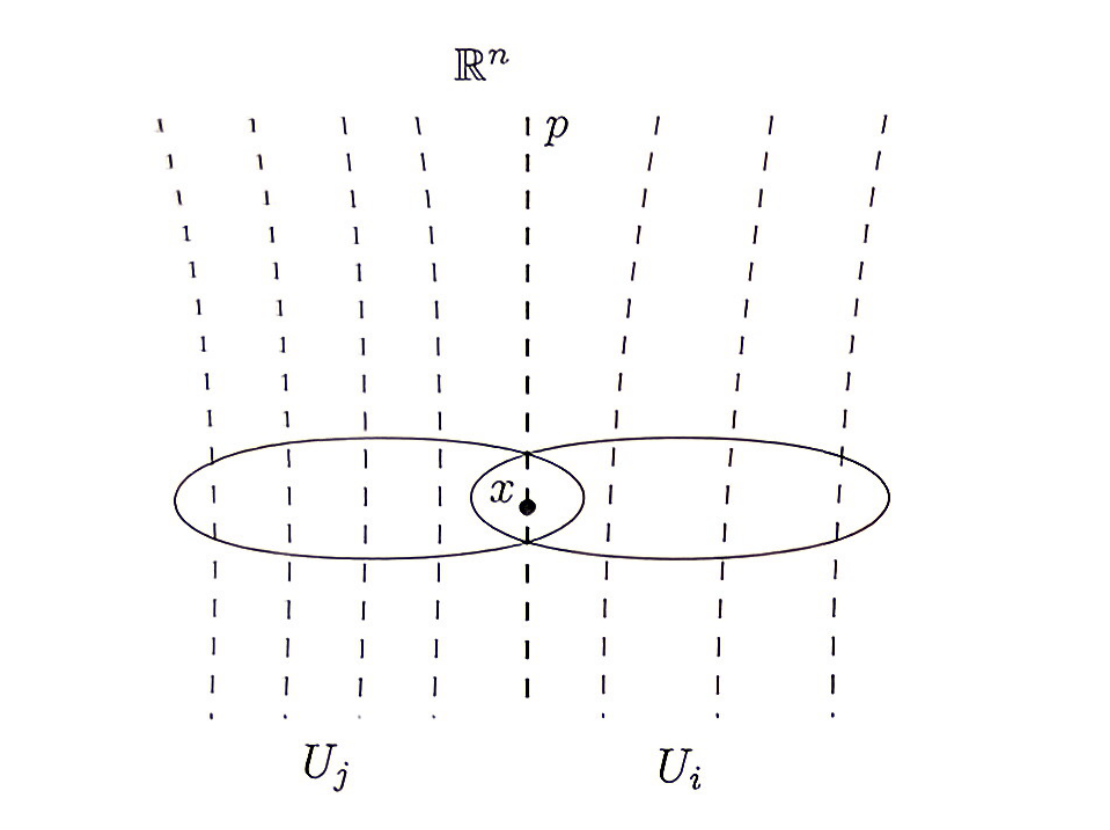
\includegraphics[width=0.60\linewidth]{figures/fig_p142_1.png}
  \caption*{图 5.21\quad 秩为 $n$ 的 $\R$-向量丛的局部图像（原书 p.134, Figure 5.21）}
\end{figure}

一般来说，这是个复杂的问题，答案严重依赖于底流形的拓扑复杂性。下面是一些容易的情形。

\begin{wexam}{5.5.1}
  取 $M=S^1$，则任何 $\R$-向量丛 $E\to S^1$ 要么平凡，要么平凡丛与 Möbius 带的直和。注意
  $E\to S^1$ 平凡当且仅当转移映射落入 $\mathrm{GL}_+(n,\R)$。\hfill$//$
\end{wexam}
% [Tutor Note: 含糊点拨——$E\to S^1$ 由单个转移矩阵 $A\in\mathrm{GL}(n,\R)$（沿 $S^1$ 的
%  和乐）的同伦类决定；$A$ 落在单位连通分支 $\mathrm{GL}_+(n,\R)$ 中当且仅当 $\det A>0$，
%  「平凡当且仅当 $\det>0$」正是这一事实的翻译。对 $n=1$ 即得「Möbius 带对应 $\det<0$」。]

\begin{wexam}{5.5.2}
  若底流形 $M$ 可缩，则任何 $\mathbf{k}$-向量丛 $E\to M$ 都平凡。我们强调：$E\to M$ 平凡的一个
  好处是它承认非零截面 $s\colon M\to E$。\hfill$//$
\end{wexam}

下面是一个更精细的问题。

\begin{wque}{5.5.2}
  已知 $E\to M$ 不是平凡向量丛，如何定量地刻画 $E\to M$ 的复杂程度？
\end{wque}

回答这个问题最有力的工具是\textbf{特征类}（characteristic class）。几乎所有的特征类都是通过
「$E\to M$ 的通有截面与零截面 $0_E$ 相交得多频繁」来定义或计算的。特别地，平凡向量丛的特征类
为零。

\begin{wexam}{5.5.3}
  在复秩为 $1$ 的 $\C$-向量丛 $E\to\CP^1$ 上，第一 Chern 类
  $c_1(E)\in H^2(\CP^1;\Z)$ 是唯一的非平凡 Chern 类。它度量的是通有截面
  $s\colon\CP^1\to E$ 与 $0_E$ 相交的带符号重数和。值 $c_1(E)([\CP^1])\in\Z$ 越大，该向量丛
  就越复杂。\hfill$//$
\end{wexam}

现在回到我们的指标故事。在辛流形 $(M^{2n},\omega)$ 上，对任何闭哈密顿轨道 $x=x(t)$，我们有秩为
$2n$ 的 $\R$-向量丛 $x^*TM\to x$，其纤维等于 $T_{x(t)}M\ (\cong\R^{2n})$，对任意
$t\in[0,1]$。重要的是，$x^*TM$ 是平凡的，因为其转移映射落在
$\mathrm{Sp}(2n)\subset\mathrm{GL}_+(2n,\R)$ 中（由练习 1.5.1 之后关于矩阵群
$\mathrm{Sp}(2n)$ 的性质 (i)）。

% >>> p143
这蕴涵存在平凡化 $x^*TM\cong S^1\times\R^{2n}$。一旦固定 $\R^{2n}$ 的一组基 $e$，它就沿整条
轨道 $x(t)$ 延拓，$t\in[0,1]$。

接下来，考虑 $T_{x(0)}M$ 在哈密顿流下的前推族，记作 $(\varphi_H^t)_*T_{x(0)}M$（见图 5.22）。
虽然作为 $2n$ 维向量空间有 $(\varphi_H^t)_*T_{x(0)}M=T_{x(t)}M$，但上面固定的基 $e$
（对每个 $t\in[0,1]$ 都放在 $T_{x(t)}M$ 中）在 $(\varphi_H^t)_*$ 的作用下可能会变化。

\begin{figure}[htbp]
  \centering
  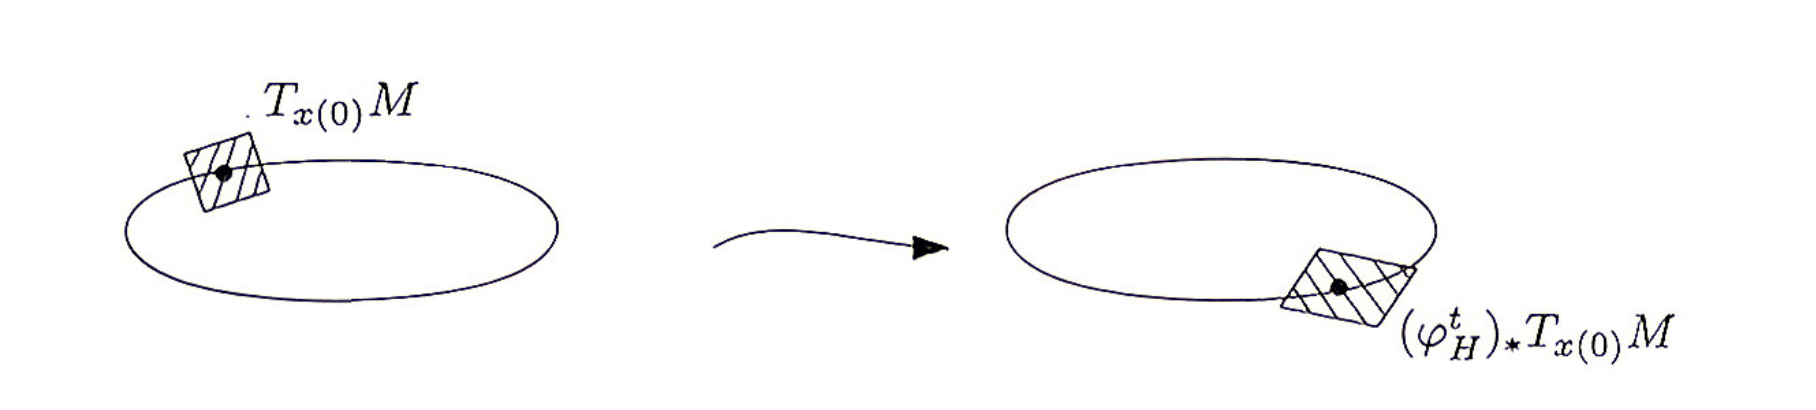
\includegraphics[width=0.82\linewidth]{figures/fig_p143_1.png}
  \caption*{图 5.22\quad $T_{x(0)}M$ 的前推（原书 p.135, Figure 5.22）}
\end{figure}

用矩阵的语言说，由于 $(\varphi_H^t)_*$ 是辛的，在基 $e$ 下前推 $\{(\varphi_H^t)_*\}_{t\in[0,1]}$
可实现为一条道路
\begin{equation}\tag{5.25}
  \{A(t)\}_{t\in[0,1]}\quad\text{in}\quad\mathrm{Sp}(2n).
\end{equation}
此外，若 $x$ 是非退化的闭哈密顿轨道，则矩阵 $A(1)$ 不以 $1$ 为特征值，因为定义 5.4.1 中的条件
此时可写成 $\det(\mathbf{1}-A(1))\ne0$。

\begin{wrem}{5.5.2}
  下面给出推导 $\mathrm{Sp}(2n)$ 中道路 $\{A(t)\}_{t\in[0,1]}$ 的另一种方式，它利用了我们这一
  情形的特殊性——闭哈密顿轨道是可缩的。对带指定界定圆盘 $(x,w)$ 的轨道，其中
  $w\colon\mathbb{D}^2\to M$，由例 5.5.2，$\R$-向量丛 $w^*TM\to\mathbb{D}^2$ 承认一个平凡化。
  再把这个平凡化限制到边界 $\partial\mathbb{D}^2$（它映到 $x$），就得到沿轨道 $x$ 的一条
  $\mathrm{Sp}(2n)$ 中的道路 $\{A(t)\}_{t\in[0,1]}$。
\end{wrem}

由目前的讨论，给闭哈密顿轨道 $x$ 指定一个指标，就归结为给 $\mathrm{Sp}(2n)$ 中的一条道路
$\{A(t)\}_{t\in[0,1]}$ 指定一个指标。下面我们以一种可计算的方式引入它，给出一个计算配方。

\textbf{第 1 步：}对每个 $t\in[0,1]$ 计算矩阵
$S(t):=-\Omega\dot A(t)A(t)^{-1}$，其中 $\Omega$ 由 (1.11) 定义。

注意 $\dot A(t)=\frac{\dd A(t)}{\dd t}=\Omega S(t)A(t)$，故 $A(t)$ 实际上是 $\Omega S(t)$ 的流。

% >>> p144
$S(t)$ 的一个重要性质是它是一个\textbf{对称矩阵}。确实，
\begin{equation*}
\begin{aligned}
  S(t)^{\mathrm T}
    &=\bigl(A(t)^{-1}\bigr)^{\mathrm T}\dot A(t)^{\mathrm T}(-\Omega)^{\mathrm T}\\
    &=\bigl(A(t)^{-1}\bigr)^{\mathrm T}\dot A(t)^{\mathrm T}\Omega\\
    &=\bigl(A(t)^{-1}\bigr)^{\mathrm T}\bigl(A(t)^{\mathrm T}\Omega\bigr)'\\
    &=\bigl(A(t)^{-1}\bigr)^{\mathrm T}\bigl(\Omega A(t)^{-1}\bigr)'\\
    &=\bigl(A(t)^{-1}\bigr)^{\mathrm T}\Omega\dot A(t)^{-1}\\
    &=\Omega A(t)\dot A(t)^{-1}\\
    &=-\Omega\dot A(t)A(t)^{-1}\\
    &=S(t).
\end{aligned}
\end{equation*}
唯一不平凡之处是：我们用了关系 $A(t)^{\mathrm T}\Omega A(t)=\Omega$（用了两次）。
% [Tutor Note: 易错预警——(1) $A\in\mathrm{Sp}(2n)$ 的定义关系是
%  $A^{\mathrm T}\Omega A=\Omega$（等价于 $A^{\mathrm T}\Omega=\Omega A^{-1}$）。干净的做法是
%  直接对它求导：$\dot A^{\mathrm T}\Omega A+A^{\mathrm T}\Omega\dot A=0$，从而
%  $S^{\mathrm T}=(A^{-1})^{\mathrm T}\dot A^{\mathrm T}(-\Omega)^{\mathrm T}
%   =-(A^{-1})^{\mathrm T}A^{\mathrm T}\Omega\dot AA^{-1}=-\Omega\dot AA^{-1}=S$。
%  按这条路线一步即可，无需经过上面链式等式的中间几步。(2) 原文链式等式的中间两行
%  （$(A^{-1})^{\mathrm T}(\Omega A^{-1})'$ 之后、以及 $(A^{-1})^{\mathrm T}\Omega\dot A^{-1}$
%  与 $\Omega A\dot A^{-1}$ 之间）按原样逐符号验证有困难，疑为排版或推导跳步；结论
%  $S(t)^{\mathrm T}=S(t)$ 本身可靠。详见 qsg/notes/review_ch05b.md。
%  (3) 记号提醒：$-\Omega$ 的转置是 $-\Omega^{\mathrm T}=\Omega$，因为 $\Omega^{\mathrm T}=-\Omega$；
%  又 $\Omega^2=-\mathbf{1}$，这些都在下一步化简中用到。]

\textbf{第 2 步：}确定道路 $\{A(t)\}_{t\in[0,1]}$ 的\textbf{交点}（crossing），即那些
$t\in[0,1]$ 使得 $\det(A(t)-\mathbf{1})=0$。然后在每个交点 $t$ 处、以及线性子空间
$\ker(A(t)-\mathbf{1})$ 上，考虑第 1 步中的对称矩阵 $S(t)$ 的限制，即
$S(t)|_{\ker(A(t)-\mathbf{1})}$，并把它看作一个双线性形式。为简洁起见，记
\begin{equation}\tag{5.26}
  \Gamma(A,t):=S(t)\big|_{\ker(A(t)-\mathbf{1})}.
\end{equation}
此外，若 $\Gamma(A,t)$ 是非退化的双线性形式，则称交点 $t$ 是\textbf{正则的}（regular）。

\begin{wexam}{5.5.4}
  按定义 $A(0)=\mathbf{1}$，故 $t=0$ 总是交点，且 $\ker(A(0)-\mathbf{1})=\R^{2n}$。假设 $t=0$
  是正则的，则 $\Gamma(A,0)$ 是整个 $\R^{2n}$ 上的非退化双线性形式。\hfill$//$
\end{wexam}

下面 (5.27) 中的事实与定义取自 [186]，它非常方便，因为它只须考虑正则交点。

\whead{事实}{5.5.1}\quad $\mathrm{Sp}(2n)$ 中的任何道路都在固定端点的意义下同伦于一条只有
正则交点的道路。特别地，对这样的道路，在闭区间 $[0,1]$ 内只有有限多个交点。

\textbf{第 3 步：}对只有正则交点的道路 $A=\{A(t)\}_{t\in[0,1]}$，计算由下式定义的
\textbf{Robin--Salamon 指标}（Robin--Salamon index）：
\begin{equation}\tag{5.27}
  \mu_{\mathrm{RS}}(A):=\frac12\sgn\bigl(\Gamma(A,0)\bigr)
    +\sum_{t\in(0,1)}\sgn\bigl(\Gamma(A,t)\bigr)
    +\frac12\sgn\bigl(\Gamma(A,1)\bigr),
\end{equation}
其中求和跑遍所有（有限多个）交点 $t$。这里，对交点 $t$ 及 (5.26) 中相应的（非退化）双线性形式，
\[
  \sgn\bigl(\Gamma(A,t)\bigr)
    =\#\{\Gamma(A,t)\text{ 的正特征值}\}-\#\{\Gamma(A,t)\text{ 的负特征值}\}.
\]
注意 (5.27) 中的取值可能是半整数，即属于 $\frac12\Z$。
% [Tutor Note: 易错预警——(1) 端点 $t=0$ 与 $t=1$ 各带系数 $\tfrac12$，而内点 $t\in(0,1)$
%  的系数为 $1$；若把端点也按系数 $1$ 计，$\mu_{\mathrm{RS}}$ 就不再是同伦不变量。(2) $\sgn$
%  这里指对称双线性形式的符号差（正、负惯性指数之差），不是矩阵符号；$\Gamma(A,t)$ 只在
%  $\ker(A(t)-\mathbf{1})$ 上定义，故 $\sgn$ 也只在那个子空间上取。(3) 原文 Fact 5.5.1 只
%  断言「可同伦到只有正则交点的道路」，并未证明；其证明要用 $\mathrm{Sp}(2n)$ 中交点的
%  横截性（Bott 型论证），见 [186]。]

% >>> p145
重要的是，指标 $\mu_{\mathrm{RS}}(\cdot)$ 在固定端点的同伦下是不变的（在只有正则交点的道路之间），
故对任何道路 $A\in\mathrm{Sp}(2n)$ 定义 $\mu_{\mathrm{RS}}(A)$ 是合理的——只须在 $A$ 的同伦类中
任取一条只有正则交点的道路并按 (5.27) 计算。

\begin{wexam}{5.5.5}
  若从 $A(0)=\mathbf{1}$ 出发的道路 $A=\{A(t)\}_{t\in[0,1]}$ 满足条件：$A(1)$ 不以 $1$ 为
  特征值（因此 $1$ 不是交点，且 $\ker(A(1)-\mathbf{1})=\{0\}\subset\R^{2n}$），则
  \begin{equation*}
  \begin{aligned}
    \mu_{\mathrm{RS}}(A)
      &=\frac12\sgn\bigl(\Gamma(A,0)\bigr)
        +\sum_{t\in(0,1)}\sgn\bigl(\Gamma(A,t)\bigr)
        +\frac12\sgn\bigl(\Gamma(A,1)\bigr)\\
      &=\frac12\sgn\bigl(\Gamma(A,0)\bigr)
        +\sum_{t\in(0,1)}\sgn\bigl(\Gamma(A,t)\bigr)\\
      &=\frac12\cdot(\text{一个偶数})
        +\sum_{t\in(0,1)}\sgn\bigl(\Gamma(A,t)\bigr)\in\Z.
  \end{aligned}
  \end{equation*}
  最后一个等式来自例 5.5.4，那里 $\sgn(\Gamma(A,0))$ 与 $2n$（偶数）有相同的奇偶性。\hfill$//$
\end{wexam}

\begin{wexam}{5.5.6}
  若 $A=\{A(t)\}_{t\in[0,1]}$ 是 $\mathrm{Sp}(2n)$ 中以 $\mathbf{1}$ 为基点的环路（特别地
  $A(0)=A(1)=\mathbf{1}$），则
  \begin{equation*}
  \begin{aligned}
    \mu_{\mathrm{RS}}(A)
      &=\frac12\sgn\bigl(\Gamma(A,0)\bigr)
        +\sum_{t\in(0,1)}\sgn\bigl(\Gamma(A,t)\bigr)
        +\frac12\sgn\bigl(\Gamma(A,1)\bigr)\\
      &=2\cdot\frac12\sgn\bigl(\Gamma(A,0)\bigr)
        +\sum_{t\in(0,1)}\sgn\bigl(\Gamma(A,t)\bigr)\in\Z.
  \end{aligned}
  \end{equation*}
  这个由 $\mu_{\mathrm{RS}}$ 得到的计算结果，历史上被称为环路 $A$ 的\textbf{Maslov 指标}。
  \hfill$//$
\end{wexam}

现在，综合迄今为止讨论的一切，下面是可赋予闭哈密顿轨道的指标。

\begin{wdefn}{5.5.1}
  给定辛流形 $(M,\omega)$ 与哈密顿函数 $H\colon M\times[0,1]\to\R$，对哈密顿流
  $\{\varphi_H^t\}_{t\in[0,1]}$ 的一条非退化闭哈密顿轨道 $x=x(t)$，定义其
  \textbf{Conley--Zehnder 指标}为
  \[
    \mu_{\mathrm{CZ}}(x):=\mu_{\mathrm{RS}}(A),
  \]
  其中 $A=\{A(t)\}_{t\in[0,1]}$ 是沿轨道 $x$ 把前推 $(\varphi_H^t)_*$ 平凡化之后 (5.25) 中的
  那条辛矩阵道路。
\end{wdefn}

\begin{wrem}{5.5.3}
  (i) 由例 5.5.5，闭哈密顿轨道 $x$ 的非退化性蕴涵 $\mu_{\mathrm{CZ}}(x)$ 总是整数。
  (ii) 严格地说，矩阵 $A(t)$ 依赖于所选的初始基 $e$（比如取 $x(0)$ 处纤维 $\R^{2n}$ 的一组基）。
  基的不同选取给出另一条矩阵道路 $\{B(t)\}_{t\in[0,1]}$，它与 $\{A(t)\}_{t\in[0,1]}$ 逐时刻
  共轭。由 [186]，$\mu_{\mathrm{RS}}$ 在共轭下也不变。
\end{wrem}
% [Tutor Note: 术语依据——Conley--Zehnder 指标（Conley--Zehnder index，1984）与
%  Robin--Salamon 指标（Robin--Salamon，1993）是同一族指标的两种规范化；本书用后者定义前者，
%  是因为 Robin--Salamon 的版本对任意 $\mathrm{Sp}(2n)$ 道路（不必来自哈密顿系统、也不必非退化）
%  都有定义，且在半整数取值上自然。请注意 $\mu_{\mathrm{CZ}}$ 依赖 $H$ 的选取（它由
%  $(\varphi_H^t)_*$ 决定），但沿轨道 $x$ 的指标在 $H$ 作定常扰动时只按一个常数平移。]

% >>> p146
下面我们显式地计算一条简单但标准的辛矩阵道路的 Conley--Zehnder 指标。

\begin{wexam}{5.5.7}
  在 $(\R^2,\omega_{\mathrm{std}})$ 上考虑哈密顿函数 $H(x,y)=\frac{3\pi}{2}(x^2+y^2)$。这是一个
  Morse 函数，其唯一临界点是 $0$，且 Morse 指标为 $0$。同时，点 $0$ 也可以看作一条（常值的）
  闭哈密顿轨道。确实，
  \[
    X_H(x,y)=-3\pi y\frac{\partial}{\partial x}+3\pi x\frac{\partial}{\partial y},
  \]
  这表明除 $0\in\R^2$ 之外，其他所有点都在（以旋转的方式）运动，并且在时刻 $t=1$ 不会回到
  自身（见练习 1.7.1）。更具体地，哈密顿流由下式给出：
  \begin{equation}\tag{5.28}
    \varphi_H^t(x,y)=\bigl(\cos(3\pi t)x-\sin(3\pi t)y,\
      \sin(3\pi t)x+\cos(3\pi t)y\bigr).
  \end{equation}

  按上面的步骤，我们来计算这条位于 $0$ 的常值轨道的 $\mu_{\mathrm{CZ}}$。由于 $\varphi_H^t$
  已经是线性的，对任意 $t\in[0,1]$，前推
  $(\varphi_H^t)_*\colon T_0\R^2\to T_0\R^2$ 在标准基 $(\partial_x,\partial_y)$ 下由下述矩阵
  表示：
  \[
    A(t)=\begin{pmatrix}
      \cos(3\pi t) & -\sin(3\pi t)\\
      \sin(3\pi t) & \cos(3\pi t)
    \end{pmatrix}.
  \]
  注意
  \[
    A(1)=\begin{pmatrix}-1&0\\0&-1\end{pmatrix},
  \]
  因此，$0$ 作为轨道在定义 5.4.1 的意义下是非退化的。

  \textbf{第 1 步：}计算对称矩阵 $S(t)$。
  \begin{equation*}
  \begin{aligned}
    S(t)&=-\Omega\dot A(t)A(t)^{-1}\\
      &=\begin{pmatrix}0&1\\-1&0\end{pmatrix}
        \begin{pmatrix}-3\pi\sin(3\pi t)&-3\pi\cos(3\pi t)\\
                       3\pi\cos(3\pi t)&-3\pi\sin(3\pi t)\end{pmatrix}
        \begin{pmatrix}\cos(3\pi t)&\sin(3\pi t)\\
                       -\sin(3\pi t)&\cos(3\pi t)\end{pmatrix}\\
      &=3\pi\cdot\begin{pmatrix}0&1\\-1&0\end{pmatrix}
        \begin{pmatrix}0&-1\\1&0\end{pmatrix}
       =\begin{pmatrix}3\pi&0\\0&3\pi\end{pmatrix}.
  \end{aligned}
  \end{equation*}
  有趣的是，它对所有 $t\in[0,1]$ 都是常值且非退化的。

  \textbf{第 2 步：}对道路 $A=\{A(t)\}_{t\in[0,1]}$，有两个交点，分别出现在时刻 $t=0$ 与
  $t=\frac23$（见图 5.23）。交点 $t=0$ 与 $t=\frac23$ 都是正则的。

  \textbf{第 3 步：}按 (5.27) 计算 Robin--Salamon 指标：
  \begin{equation*}
  \begin{aligned}
    \mu_{\mathrm{RS}}(A)
      &=\frac12\sgn\bigl(\Gamma(A,0)\bigr)
        +\sum_{t\in(0,1)}\sgn\bigl(\Gamma(A,t)\bigr)
        +\frac12\sgn\bigl(\Gamma(A,1)\bigr)\\
      &=\frac12\cdot2+2=3.
  \end{aligned}
  \end{equation*}

  \hfill$//$
\end{wexam}
% [Tutor Note: 易错预警——第 3 步中 $\Gamma(A,0)$ 与 $\Gamma(A,\frac23)$ 都等于 $3\pi\,\mathbf{1}$
%  （限制在各自核上），故各自符号差为 $2$；而 $t=1$ 不是交点（$A(1)=-1$ 无特征值 $1$），
%  端点项 $\tfrac12\sgn(\Gamma(A,1))$ 消失。于是 $\mu_{\mathrm{RS}}=\tfrac12\cdot2+2=3$。
%  请务必区分「$\det(A(t)-\mathbf{1})=0$ 的时刻」与「$A(t)$ 的特征值」：$t=2/3$ 时
%  $A(2/3)=\mathbf{1}$，恰是交点；$t=1/3$ 时 $A(1/3)$ 是旋转 $90^\circ$，并非交点。]

% >>> p147
\begin{figure}[htbp]
  \centering
  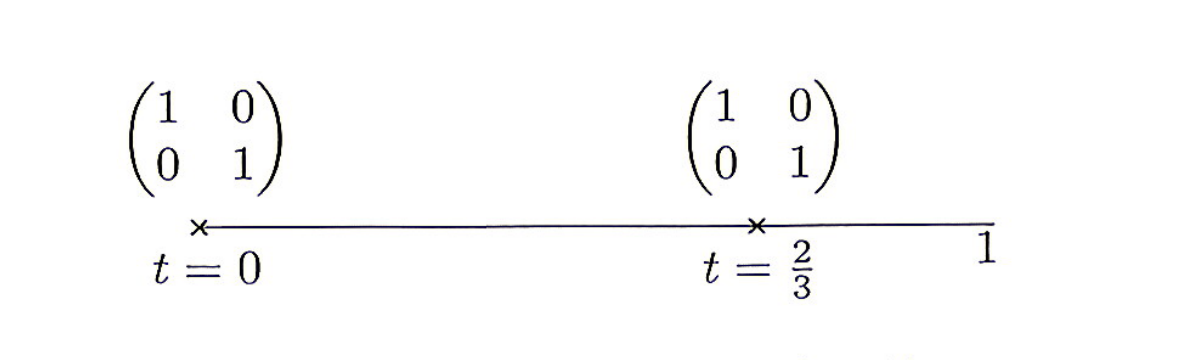
\includegraphics[width=0.62\linewidth]{figures/fig_p147_1.png}
  \caption*{图 5.23\quad 道路 $A=\{A(t)\}_{t\in[0,1]}$ 的交点（原书 p.139, Figure 5.23）}
\end{figure}

因此，$\mu_{\mathrm{CZ}}(0)=\mu_{\mathrm{RS}}(A)=3$。注意 $\mu_{\mathrm{CZ}}(0)$ 与 Morse 指标
$\ind_H(0)$ 并不一致！

\begin{wrem}{5.5.4}
  即使 $\alpha$ 足够小、使得 $t=0$ 是唯一的正则交点，仍然有 $\mu_{\mathrm{CZ}}(0)=1\ne0=\ind_H(0)$。
  有时会加入一个规范化来消除这种不一致。例如，定义一个新的（规范化的）Conley--Zehnder 指标
  $n-\mu_{\mathrm{CZ}}$，其中 $n=\frac12\dim(M)$。
\end{wrem}
% [Tutor Note: 含糊点拨——注 5.5.4 出现在练习 5.5.1 之前，其中的 $\alpha$ 指的是紧接着的
%  练习 5.5.1 中 $H=\pi\alpha(x^2+y^2)$ 的参数；原文把注放在练习之前，阅读时应先看练习。
%  该练习的答案是 $\mu_{\mathrm{CZ}}(0)=2\lfloor\alpha\rfloor+1$（对 $\alpha>0$ 且
%  $\alpha\notin\Z$）：交点为 $t=k/\alpha$（$k=0,1,\dots,\lfloor\alpha\rfloor$），每处
%  $\sgn\Gamma=2$，故 $\mu_{\mathrm{RS}}=\frac12\cdot2+2\lfloor\alpha\rfloor$。取
%  $0<\alpha<1$ 即得 $1$，与注 5.5.4 相符。]

\begin{wexer}{5.5.1}
  在 $(\R^2,\omega_{\mathrm{std}})$ 上考虑哈密顿函数
  \[
    H(x,y)=\pi\alpha(x^2+y^2),
  \]
  其中 $\alpha\notin\R/\Z$。仿照例 5.5.7，把 $0$ 看作哈密顿流 $\{\varphi_H^t\}_{t\in[0,1]}$ 的
  闭轨道，计算它的 Conley--Zehnder 指标 $\mu_{\mathrm{CZ}}(0)$，并把它写成 $\alpha$ 的表达式。
\end{wexer}

\begin{wexer}{5.5.2}（[107] 中的命题 4.9）
  考虑由下述\textbf{辛剪切矩阵}（symplectic shear matrix）给出的矩阵道路
  $A=\{A(t)\}_{t\in[0,1]}$：
  \[
    A(t)=\begin{pmatrix}\mathbf{1}&B(t)\\ 0&\mathbf{1}\end{pmatrix}\in\mathrm{Sp}(2n),
  \]
  其中 $B(t)$ 是 $n\times n$ 对称矩阵。计算 $\mu_{\mathrm{RS}}(A)$。（提示：注意这是一条高度
  退化的道路，故需要构造一个扰动，使所得道路只有非退化的正则交点。）
\end{wexer}

\begin{wrem}{5.5.5}
  对带界定圆盘 $w$ 的闭哈密顿轨道 $x$，注 5.5.2 提示了另一种得到平凡化、从而得到
  $\mathrm{Sp}(2n)$ 中辛矩阵道路的方式。确切地说，沿 $x$ 的平凡化来自沿圆盘 $w$ 的平凡化的
  限制。由 $\mathbb{D}^2$ 的可缩性，固定界定圆盘 $w$ 的两个平凡化将诱导出 $\mathrm{Sp}(2n)$ 中
  两条在固定端点下同伦的道路 $A$、$A'$。这意味着可以把带盖轨道 $(x,w)$ 的 Conley--Zehnder
  指标——记作 $\mu_{\mathrm{CZ}}((x,w))$——定义为任一这样诱导出的辛矩阵道路的
  Robin--Salamon 指标 $\mu_{\mathrm{RS}}$（见 (5.27)）。
\end{wrem}

然而，一旦更换界定圆盘，沿 $w$ 与 $w'$ 的平凡化可能诱导出 $\mathrm{Sp}(2n)$ 中不同伦的道路，
这将可能改变 $\mu_{\mathrm{CZ}}((x,w))$ 的值。与关于辛作用量泛函 $\mathcal{A}_H$ 可能变化的
讨论（就在命题 5.4.1 之前）类似，
% >>> p148
当选择不同的界定圆盘时，差别将由拓扑 $2$-球面 $\overline{w}\#w'$ 给出（见图 5.16）。下面是
[195] 中的一个标准结果，它刻画了更换界定圆盘时的影响：
\[
  \mu_{\mathrm{CZ}}\bigl((x,w)\bigr)-\mu_{\mathrm{CZ}}\bigl((x,w')\bigr)
    =2c_1\bigl(\overline{w}\#w'\bigr).
\]
在辛非球面情形，由 (5.16) 中关于第一 Chern 类的第二个条件，我们有
$\mu_{\mathrm{CZ}}((x,w))=\mu_{\mathrm{CZ}}((x,w'))$。
% [Tutor Note: 易错预警——$c_1(\overline{w}\#w')$ 是 Chern 类在球面类上的配对，前面系数
%  $2$ 来自 Maslov 类与第一 Chern 类的换算（Maslov 指标按 $\pi_1(\mathrm{U}(n))=\Z$ 规范化，
%  而 $c_1$ 的配对在拉回后相差因子 $2$）；不同文献对 $\mu_{\mathrm{CZ}}$ 的规范化不同，
%  系数可能是 $2$ 也可能是 $1$，引用时须核对该文献的约定。另请与 (5.18) 之前的讨论对照：
%  作用量泛函的差别是 $\int_{\overline{w}\#w'}\omega$，指标的差别则是 $2c_1$；在辛非球面
%  条件下二者都消失，这正是 Floer 理论在辛非球面情形能顺利定义的原因。]
